\documentclass[11pt,addpoints,answers]{exam}

%-----------------------------------------------------------------------------
% PACKAGES AND OTHER DOCUMENT CONFIGURATIONS
%-----------------------------------------------------------------------------

\usepackage[margin=1in]{geometry}
\usepackage{amsmath, amsfonts}
\usepackage{enumerate}
\usepackage{graphicx}
\usepackage{titling}
\usepackage{url}
\usepackage{xfrac}
\usepackage{natbib}
\usepackage{amssymb}
\usepackage{amsthm}
\usepackage{paralist}
\usepackage{epstopdf}
\usepackage{tabularx}
\usepackage{longtable}
\usepackage{multirow}
\usepackage{multicol}
\usepackage[colorlinks=true,urlcolor=blue]{hyperref}
\usepackage{algorithm}
\usepackage{algorithmicx}
\usepackage[noend]{algpseudocode}
\usepackage{float}
\usepackage{enumerate}
\usepackage{array}
\usepackage{environ}
\usepackage{times}
\usepackage{textcomp}
\usepackage{caption}
\usepackage{parskip} % For NIPS style paragraphs.
\usepackage[compact]{titlesec} % Less whitespace around titles
\usepackage[inline]{enumitem} % For inline enumerate* and itemize*
\usepackage{datetime}
\usepackage{comment}
% \usepackage{minted}
\usepackage{lastpage}
\usepackage{color}
\usepackage{xcolor}
\usepackage[final]{listings}
\usepackage{tikz}
\usetikzlibrary{shapes,decorations}
\usepackage{framed}
\usepackage{booktabs}
\usepackage{cprotect}
\usepackage{verbatimbox}
\usepackage{multicol}
\usepackage{hyperref}
\usepackage{subcaption}
\usepackage{mathtools} % For drcases
\usepackage{cancel}
\usepackage[many]{tcolorbox}
\usepackage{soul}
\usepackage[bottom]{footmisc}
\usepackage{bm}
\usepackage{wasysym}

\usepackage{tikz}
\usetikzlibrary{shapes.geometric}
\usetikzlibrary{positioning, arrows, automata}

\newtcolorbox[]{your_solution}[1][]{%
    % breakable,
    enhanced,
    nobeforeafter,
    colback=white,
    title=Your Answer,
    sidebyside align=top,
    box align=top,
    #1
}

%%%%%%%%%%%%%%%%%%%%%%%%%%%%%%%%%%%%%%%%%%%
% Rotated Column Headers                  %
%%%%%%%%%%%%%%%%%%%%%%%%%%%%%%%%%%%%%%%%%%%
\usepackage{adjustbox}
\usepackage{array}

%https://tex.stackexchange.com/questions/32683/rotated-column-titles-in-tabular

\newcolumntype{R}[2]{%
    >{\adjustbox{angle=#1,lap=\width-(#2)}\bgroup}%
    l%
    <{\egroup}%
}
\newcommand*\rot{\multicolumn{1}{R{45}{1em}}}% no optional argument here, please!


%%%%%%%%%%%%%%%%%%%%%%%%%%%%%%%%%%%%%%%%%%%
% Better numbering                        %
%%%%%%%%%%%%%%%%%%%%%%%%%%%%%%%%%%%%%%%%%%%

% \numberwithin{equation}{section} % Number equations within sections (i.e. 1.1, 1.2, 2.1, 2.2 instead of 1, 2, 3, 4)
% \numberwithin{figure}{section} % Number figures within sections (i.e. 1.1, 1.2, 2.1, 2.2 instead of 1, 2, 3, 4)
% \numberwithin{table}{section} % Number tables within sections (i.e. 1.1, 1.2, 2.1, 2.2 instead of 1, 2, 3, 4)

%%%%%%%%%%%%%%%%%%%%%%%%%%%%%%%%%%%%%%%%%%
% Custom commands                        %
%%%%%%%%%%%%%%%%%%%%%%%%%%%%%%%%%%%%%%%%%%

\newcommand{\vc}[1]{\boldsymbol{#1}}
\newcommand{\adj}[1]{\frac{d J}{d #1}}
\newcommand{\chain}[2]{\adj{#2} = \adj{#1}\frac{d #1}{d #2}}

\newcommand{\independent}{\perp\!\!\!\perp  }

\newcommand{\R}{\mathbb{R}}
\newcommand{\blackcircle}{\tikz\draw[black,fill=black] (0,0) circle (1ex);}
\renewcommand{\circle}{\tikz\draw[black] (0,0) circle (1ex);}

\newcommand{\emptysquare}{{\LARGE $\square$}\ \ }
\newcommand{\filledsquare}{{\LARGE $\boxtimes$}\ \ }
\newcommand{\emptycircle}{{\LARGE $\fullmoon$}\ \ }
\newcommand{\filledcircle}{{\LARGE $\newmoon$}\ \ }


% mathcal
\newcommand{\Ac}{\mathcal{A}}
\newcommand{\Bc}{\mathcal{B}}
\newcommand{\Cc}{\mathcal{C}}
\newcommand{\Dc}{\mathcal{D}}
\newcommand{\Ec}{\mathcal{E}}
\newcommand{\Fc}{\mathcal{F}}
\newcommand{\Gc}{\mathcal{G}}
\newcommand{\Hc}{\mathcal{H}}
\newcommand{\Ic}{\mathcal{I}}
\newcommand{\Jc}{\mathcal{J}}
\newcommand{\Kc}{\mathcal{K}}
\newcommand{\Lc}{\mathcal{L}}
\newcommand{\Mc}{\mathcal{M}}
\newcommand{\Nc}{\mathcal{N}}
\newcommand{\Oc}{\mathcal{O}}
\newcommand{\Pc}{\mathcal{P}}
\newcommand{\Qc}{\mathcal{Q}}
\newcommand{\Rc}{\mathcal{R}}
\newcommand{\Sc}{\mathcal{S}}
\newcommand{\Tc}{\mathcal{T}}
\newcommand{\Uc}{\mathcal{U}}
\newcommand{\Vc}{\mathcal{V}}
\newcommand{\Wc}{\mathcal{W}}
\newcommand{\Xc}{\mathcal{X}}
\newcommand{\Yc}{\mathcal{Y}}
\newcommand{\Zc}{\mathcal{Z}}

% mathbb
\newcommand{\Ab}{\mathbb{A}}
\newcommand{\Bb}{\mathbb{B}}
\newcommand{\Cb}{\mathbb{C}}
\newcommand{\Db}{\mathbb{D}}
\newcommand{\Eb}{\mathbb{E}}
\newcommand{\Fb}{\mathbb{F}}
\newcommand{\Gb}{\mathbb{G}}
\newcommand{\Hb}{\mathbb{H}}
\newcommand{\Ib}{\mathbb{I}}
\newcommand{\Jb}{\mathbb{J}}
\newcommand{\Kb}{\mathbb{K}}
\newcommand{\Lb}{\mathbb{L}}
\newcommand{\Mb}{\mathbb{M}}
\newcommand{\Nb}{\mathbb{N}}
\newcommand{\Ob}{\mathbb{O}}
\newcommand{\Pb}{\mathbb{P}}
\newcommand{\Qb}{\mathbb{Q}}
\newcommand{\Rb}{\mathbb{R}}
\newcommand{\Sb}{\mathbb{S}}
\newcommand{\Tb}{\mathbb{T}}
\newcommand{\Ub}{\mathbb{U}}
\newcommand{\Vb}{\mathbb{V}}
\newcommand{\Wb}{\mathbb{W}}
\newcommand{\Xb}{\mathbb{X}}
\newcommand{\Yb}{\mathbb{Y}}
\newcommand{\Zb}{\mathbb{Z}}

% mathbf lowercase
\newcommand{\av}{\mathbf{a}}
\newcommand{\bv}{\mathbf{b}}
\newcommand{\cv}{\mathbf{c}}
\newcommand{\dv}{\mathbf{d}}
\newcommand{\ev}{\mathbf{e}}
\newcommand{\fv}{\mathbf{f}}
\newcommand{\gv}{\mathbf{g}}
\newcommand{\hv}{\mathbf{h}}
\newcommand{\iv}{\mathbf{i}}
\newcommand{\jv}{\mathbf{j}}
\newcommand{\kv}{\mathbf{k}}
\newcommand{\lv}{\mathbf{l}}
\newcommand{\mv}{\mathbf{m}}
\newcommand{\nv}{\mathbf{n}}
\newcommand{\ov}{\mathbf{o}}
\newcommand{\pv}{\mathbf{p}}
\newcommand{\qv}{\mathbf{q}}
\newcommand{\rv}{\mathbf{r}}
\newcommand{\sv}{\mathbf{s}}
\newcommand{\tv}{\mathbf{t}}
\newcommand{\uv}{\mathbf{u}}
\newcommand{\vv}{\mathbf{v}}
\newcommand{\wv}{\mathbf{w}}
\newcommand{\xv}{\mathbf{x}}
\newcommand{\yv}{\mathbf{y}}
\newcommand{\zv}{\mathbf{z}}

% mathbf uppercase
\newcommand{\Av}{\mathbf{A}}
\newcommand{\Bv}{\mathbf{B}}
\newcommand{\Cv}{\mathbf{C}}
\newcommand{\Dv}{\mathbf{D}}
\newcommand{\Ev}{\mathbf{E}}
\newcommand{\Fv}{\mathbf{F}}
\newcommand{\Gv}{\mathbf{G}}
\newcommand{\Hv}{\mathbf{H}}
\newcommand{\Iv}{\mathbf{I}}
\newcommand{\Jv}{\mathbf{J}}
\newcommand{\Kv}{\mathbf{K}}
\newcommand{\Lv}{\mathbf{L}}
\newcommand{\Mv}{\mathbf{M}}
\newcommand{\Nv}{\mathbf{N}}
\newcommand{\Ov}{\mathbf{O}}
\newcommand{\Pv}{\mathbf{P}}
\newcommand{\Qv}{\mathbf{Q}}
\newcommand{\Rv}{\mathbf{R}}
\newcommand{\Sv}{\mathbf{S}}
\newcommand{\Tv}{\mathbf{T}}
\newcommand{\Uv}{\mathbf{U}}
\newcommand{\Vv}{\mathbf{V}}
\newcommand{\Wv}{\mathbf{W}}
\newcommand{\Xv}{\mathbf{X}}
\newcommand{\Yv}{\mathbf{Y}}
\newcommand{\Zv}{\mathbf{Z}}

% bold greek lowercase
\newcommand{\alphav     }{\boldsymbol \alpha     }
\newcommand{\betav      }{\boldsymbol \beta      }
\newcommand{\gammav     }{\boldsymbol \gamma     }
\newcommand{\deltav     }{\boldsymbol \delta     }
\newcommand{\epsilonv   }{\boldsymbol \epsilon   }
\newcommand{\varepsilonv}{\boldsymbol \varepsilon}
\newcommand{\zetav      }{\boldsymbol \zeta      }
\newcommand{\etav       }{\boldsymbol \eta       }
\newcommand{\thetav     }{\boldsymbol \theta     }
\newcommand{\varthetav  }{\boldsymbol \vartheta  }
\newcommand{\iotav      }{\boldsymbol \iota      }
\newcommand{\kappav     }{\boldsymbol \kappa     }
\newcommand{\varkappav  }{\boldsymbol \varkappa  }
\newcommand{\lambdav    }{\boldsymbol \lambda    }
\newcommand{\muv        }{\boldsymbol \mu        }
\newcommand{\nuv        }{\boldsymbol \nu        }
\newcommand{\xiv        }{\boldsymbol \xi        }
\newcommand{\omicronv   }{\boldsymbol \omicron   }
\newcommand{\piv        }{\boldsymbol \pi        }
\newcommand{\varpiv     }{\boldsymbol \varpi     }
\newcommand{\rhov       }{\boldsymbol \rho       }
\newcommand{\varrhov    }{\boldsymbol \varrho    }
\newcommand{\sigmav     }{\boldsymbol \sigma     }
\newcommand{\varsigmav  }{\boldsymbol \varsigma  }
\newcommand{\tauv       }{\boldsymbol \tau       }
\newcommand{\upsilonv   }{\boldsymbol \upsilon   }
\newcommand{\phiv       }{\boldsymbol \phi       }
\newcommand{\varphiv    }{\boldsymbol \varphi    }
\newcommand{\chiv       }{\boldsymbol \chi       }
\newcommand{\psiv       }{\boldsymbol \psi       }
\newcommand{\omegav     }{\boldsymbol \omega     }

% bold greek uppercase
\newcommand{\Gammav     }{\boldsymbol \Gamma     }
\newcommand{\Deltav     }{\boldsymbol \Delta     }
\newcommand{\Thetav     }{\boldsymbol \Theta     }
\newcommand{\Lambdav    }{\boldsymbol \Lambda    }
\newcommand{\Xiv        }{\boldsymbol \Xi        }
\newcommand{\Piv        }{\boldsymbol \Pi        }
\newcommand{\Sigmav     }{\boldsymbol \Sigma     }
\newcommand{\Upsilonv   }{\boldsymbol \Upsilon   }
\newcommand{\Phiv       }{\boldsymbol \Phi       }
\newcommand{\Psiv       }{\boldsymbol \Psi       }
\newcommand{\Omegav     }{\boldsymbol \Omega     }

%%%%%%%%%%%%%%%%%%%%%%%%%%%%%%%%%%%%%%%%%%%
% Code highlighting with listings         %
%%%%%%%%%%%%%%%%%%%%%%%%%%%%%%%%%%%%%%%%%%%

\definecolor{bluekeywords}{rgb}{0.13,0.13,1}
\definecolor{greencomments}{rgb}{0,0.5,0}
\definecolor{redstrings}{rgb}{0.9,0,0}
\definecolor{light-gray}{gray}{0.95}

\newcommand{\MYhref}[3][blue]{\href{#2}{\color{#1}{#3}}}%

\definecolor{dkgreen}{rgb}{0,0.6,0}
\definecolor{gray}{rgb}{0.5,0.5,0.5}
\definecolor{mauve}{rgb}{0.58,0,0.82}

\lstdefinelanguage{Shell}{
  keywords={tar, cd, make},
  %keywordstyle=\color{bluekeywords}\bfseries,
  alsoletter={+},
  ndkeywords={python, py, javac, java, gcc, c, g++, cpp, .txt, octave, m, .tar},
  %ndkeywordstyle=\color{bluekeywords}\bfseries,
  identifierstyle=\color{black},
  sensitive=false,
  comment=[l]{//},
  morecomment=[s]{/*}{*/},
  commentstyle=\color{purple}\ttfamily,
  %stringstyle=\color{red}\ttfamily,
  morestring=[b]',
  morestring=[b]",
  backgroundcolor = \color{light-gray}
}

\lstset{columns=fixed, basicstyle=\ttfamily,
    backgroundcolor=\color{light-gray},xleftmargin=0.5cm,frame=tlbr,framesep=4pt,framerule=0pt}


%%%%%%%%%%%%%%%%%%%%%%%%%%%%%%%%%%%%%%%%%%%
% Custom box for highlights               %
%%%%%%%%%%%%%%%%%%%%%%%%%%%%%%%%%%%%%%%%%%%

% Define box and box title style
\tikzstyle{mybox} = [fill=blue!10, very thick,
    rectangle, rounded corners, inner sep=1em, inner ysep=1em]

% \newcommand{\notebox}[1]{
% \begin{tikzpicture}
% \node [mybox] (box){%
%     \begin{minipage}{\textwidth}
%     #1
%     \end{minipage}
% };
% \end{tikzpicture}%
% }

\NewEnviron{notebox}{

\begin{tikzpicture}
\node [mybox] (box){
    \begin{minipage}{\textwidth}
        \BODY
    \end{minipage}
};
\end{tikzpicture}
}

%%%%%%%%%%%%%%%%%%%%%%%%%%%%%%%%%%%%%%%%%%%
% Commands showing / hiding solutions     %
%%%%%%%%%%%%%%%%%%%%%%%%%%%%%%%%%%%%%%%%%%%

%% To HIDE SOLUTIONS (to post at the website for students), set this value to 0: 
\def\issoln{0}
% Some commands to allow solutions to be embedded in the assignment file.
\ifcsname issoln\endcsname \else \def\issoln{1} \fi
% Default to an empty solutions environ.
\NewEnviron{soln}{}{}
\if\issoln 1
% Otherwise, include solutions as below.
\RenewEnviron{soln}{
    \leavevmode\color{red}\ignorespaces
    % \textbf{Solution} \BODY
    \BODY
}{}
\fi

%% To HIDE TAGS set this value to 0:
\def\showtags{0}
%%%%%%%%%%%%%%%%
\ifcsname showtags\endcsname \else \def\showtags{1} \fi
% Default to an empty tags environ.
\NewEnviron{tags}{}{}
\if\showtags 1
% Otherwise, include solutions as below.
\RenewEnviron{tags}{
    \fbox{
    \leavevmode\color{blue}\ignorespaces
    \textbf{TAGS:} \texttt{\url{\BODY}}
    }
    \vspace{-.5em}
}{}
\fi

%%%%%%%%%%%%%%%%%%%%%%%%%%%%%%%%%%%%%%%%%%%
% Commands for customizing the assignment %
%%%%%%%%%%%%%%%%%%%%%%%%%%%%%%%%%%%%%%%%%%%
\newcommand{\courseNum}{10-301 / 10-601}
\newcommand{\courseName}{Introduction to Machine Learning}
\newcommand{\courseSem}{Fall 2021}
\newcommand{\courseUrl}{\url{http://mlcourse.org}}
\newcommand{\hwNum}{Homework 8}
\newcommand{\hwTopic}{Reinforcement Learning}
\newcommand{\hwName}{\hwNum: \hwTopic}
\newcommand{\outDate}{Nov. 12, 2021}
\newcommand{\dueDate}{Nov. 21, 2021}
\newcommand{\taNames}{Gopi Krishna, Roshan, Justin, Youngjoo, Jingyun}


%\pagestyle{fancyplain}
\newcommand{\homeworktype}{\string written/programming}
\lhead{\hwName}
\rhead{\courseNum}
\cfoot{\thepage{} of \numpages{}}

\title{\textsc{\hwNum}\\
\textsc{\hwTopic}
\thanks{Compiled on \today{} at \currenttime{}}\\
\vspace{1em}
} % Title


\author{\textsc{\large \courseNum{} \courseName{} (\courseSem)}\\
\courseUrl
\vspace{1em}\\
  OUT: \outDate \\
  DUE: \dueDate \\
  TAs: \taNames\\
}

\date{}

%%%%%%%%%%%%%%%%%%%%%%%%%%%%%%%%%%%%%%%%%%%%%%%%%
% Useful commands for typesetting the questions %
%%%%%%%%%%%%%%%%%%%%%%%%%%%%%%%%%%%%%%%%%%%%%%%%%

\newcommand \expect {\mathbb{E}}
\newcommand \mle [1]{{\hat #1}^{\rm MLE}}
\newcommand \map [1]{{\hat #1}^{\rm MAP}}
\newcommand \argmax {\operatorname*{argmax}}
\newcommand \argmin {\operatorname*{argmin}}
\newcommand \code [1]{{\tt #1}}
\newcommand \datacount [1]{\#\{#1\}}
\newcommand \ind [1]{\mathbb{I}\{#1\}}

%%%%%%%%%%%%%%%%%%%%%%%%%%
% Document configuration %
%%%%%%%%%%%%%%%%%%%%%%%%%%

% Don't display a date in the title and remove the white space
\predate{}
\postdate{}
\date{}

% Don't display an author and remove the white space
%\preauthor{}
%\postauthor{}

%%%%%%%%%%%%%%%%%%
% Begin Document %
%%%%%%%%%%%%%%%%%% 

\usepackage{scalerel, amssymb}

\def\rr{{\color{red}$\mathrel{\bigcirc}$}}
\def\bb{{\color{blue}$\mathrel{\bigcirc}$}}

\begin{document}

\maketitle

\begin{notebox}
\paragraph{Summary} In this assignment, you will implement a reinforcement learning algorithm for solving the classic mountain-car environment. As a warmup, the first section will lead you through an on-paper example of how value iteration and Q-learning work. Then, in Section \ref{sec:code}, you will implement Q-learning with function approximation to solve the mountain car environment.
\end{notebox}\newcommand \maxsubs {10 }
\section*{START HERE: Instructions}
\begin{itemize}

\item \textbf{Collaboration Policy}: Please read the collaboration policy here: \url{http://www.cs.cmu.edu/~mgormley/courses/10601/syllabus.html}

\item\textbf{Late Submission Policy:} See the late submission policy here: \url{http://www.cs.cmu.edu/~mgormley/courses/10601/syllabus.html}

\item\textbf{Submitting your work:} You will use Gradescope to submit
  answers to all questions and code. Please
  follow instructions at the end of this PDF to correctly submit all your code to Gradescope.

  \begin{itemize}
    
 % COMMENT IF NOT USING CANVAS
\begin{comment}
  \item \textbf{Canvas:} Canvas (\url{https://canvas.cmu.edu}) will be
    used for quiz-style problems (e.g. multiple choice, true / false,
    numerical answers). Grading is done automatically.
    %
    You may only \textbf{submit once} on canvas, so be sure of your
    answers before you submit. However, canvas allows you to work on
    your answers and then close out of the page and it will save your
    progress.  You will not be granted additional submissions, so
    please be confident of your solutions when you are submitting your
    assignment.
    %
    {\color{red} The above is true for future assignments, but this one
    allows {\bf unlimited submissions}.}
\end{comment}
    
  % COMMENT IF NOT USING GRADESCOPE
   \item \textbf{Written:} For written problems such as short answer, multiple choice, derivations, proofs, or plots, please use the provided template. Submissions can be handwritten onto the template, but should be labeled and clearly legible. If your writing is not legible, you will not be awarded marks. If your scanned submission misaligns the template, there will be a 5\% penalty. Alternatively, submissions can be written in LaTeX. 
   Each derivation/proof should be completed in the boxes provided. If you do not follow the template, your assignment may not be graded correctly by our AI assisted grader.

  %   COMMENT IF NOT USING GRADESCOPE AUTOGRADER
  \ifthenelse{\equal{\homeworktype}{\string written}}{}{
\item \textbf{Programming:} You will submit your code for programming questions on the homework to Gradescope (\url{https://gradescope.com}). After uploading your code, our grading scripts will autograde your assignment by running your program on a virtual machine (VM). When you are developing, check that the version number of the programming language environment (e.g. Python 3.9.6, OpenJDK 11.0.11, g++ 7.5.0) and versions of permitted libraries (e.g.  \texttt{numpy} 1.21.2 and \texttt{scipy} 1.7.1) match those used on Gradescope. You have \maxsubs free Gradescope programming submissions. After \maxsubs submissions, you will begin to lose points from your total programming score. We recommend debugging your implementation on your local machine (or the Linux servers) and making sure your code is running correctly first before submitting your code to Gradescope.}

  \end{itemize}
  
\ifthenelse{\equal{\homeworktype}{\string written}}{}{\item\textbf{Materials:} The data that you will need in order to complete this assignment is posted along with the writeup and template on the course website.}

\end{itemize}


\ifthenelse{\equal{\homeworktype}{\string written}}{}{\begin{notebox}
\paragraph{Linear Algebra Libraries} When implementing machine learning algorithms, it is often convenient to have a linear algebra library at your disposal. In this assignment, Java users may use EJML\footnote{\url{https://ejml.org}} or ND4J\footnote{\url{https://javadoc.io/doc/org.nd4j/nd4j-api/latest/index.html}} and C++ users may use Eigen\footnote{\url{http://eigen.tuxfamily.org/}}. Details below. 
%
(As usual, Python users have NumPy.)
%
\begin{description}
\item[EJML for Java] EJML is a pure Java linear algebra package with three interfaces. We strongly recommend using the SimpleMatrix interface. The autograder will use EJML version 0.41. When compiling and running your code, we will add the additional command line argument {\footnotesize{\lstinline{-cp "linalg_lib/ejml-v0.41-libs/*:linalg_lib/nd4j-v1.0.0-M1.1-libs/*:./"}}}
to ensure that all the EJML jars are on the classpath as well as your code. 

\item[ND4J for Java] ND4J is a library for multidimensional tensors with an interface akin to Python's NumPy. The autograder will use ND4J version 1.0.0-M1.1. When compiling and running your code, we will add the additional command line argument {\footnotesize{\lstinline{-cp "linalg_lib/ejml-v0.41-libs/*:linalg_lib/nd4j-v1.0.0-M1.1-libs/*:./"}}} to ensure that all the ND4J jars are on the classpath as well as your code. 

\item[Eigen for C++] Eigen is a header-only library, so there is no linking to worry about---just \lstinline{#include} whatever components you need. The autograder will use Eigen version 3.4.0. The command line arguments above demonstrate how we will call you code. When compiling your code we will include, the argument \lstinline{-I./linalg_lib} in order to include the \lstinline{linalg_lib/Eigen} subdirectory, which contains all the headers.

\end{description} 
We have included the correct versions of EJML/ND4J/Eigen in the \lstinline{linalg_lib.zip} posted on the Coursework page of the course website for your convenience. It contains the same \lstinline{linalg_lib/} directory that we will include in the current working directory when running your tests. Do {\bf not} include EJML, ND4J, or Eigen in your homework submission; the autograder will ensure that they are in place. 
\end{notebox}}\clearpage

\section*{Instructions for Specific Problem Types}

For ``Select One" questions, please fill in the appropriate bubble completely:

\begin{quote}
\textbf{Select One:} Who taught this course?
\begin{list}{}
     \item\CIRCLE{} Matt Gormley / Henry Chai
     \item\Circle{} Marie Curie
     \item\Circle{} Noam Chomsky
\end{list}
\end{quote}


If you need to change your answer, you may cross out the previous answer and bubble in the new answer:

\begin{quote}
\textbf{Select One:} Who taught this course?
\begin{list}{}
     \item\CIRCLE{} Matt Gormley / Henry Chai
     \item\Circle{} Marie Curie\\
     \xcancel{\CIRCLE}{} Noam Chomsky
\end{list}
\end{quote}


For ``Select all that apply" questions, please fill in all appropriate squares completely:

\begin{quote}
\textbf{Select all that apply:} Which are scientists?
{
    \checkboxchar{$\Box$} \checkedchar{$\blacksquare$}
    \begin{checkboxes}
     \choice Stephen Hawking 
     \CorrectChoice Albert Einstein
     \choice Isaac Newton
     \choice None of the above
    \end{checkboxes}
    }
\end{quote}

Again, if you need to change your answer, you may cross out the previous answer(s) and bubble in the new answer(s):

\begin{quote}
\textbf{Select all that apply:} Which are scientists?
    \begin{list}{}
    \item $\blacksquare$ Stephen Hawking 
    \item $\blacksquare$ Albert Einstein
    \item $\blacksquare$ Isaac Newton\\
    \xcancel{$\blacksquare$} I don't know
\end{list}
\end{quote}

For questions where you must fill in a blank, please make sure your final answer is fully included in the given space. You may cross out answers or parts of answers, but the final answer must still be within the given space.

\begin{quote}
\textbf{Fill in the blank:} What is the course number?

\begin{tcolorbox}[fit,height=1cm, width=4cm, blank, borderline={1pt}{-2pt},nobeforeafter]
    \begin{center}\huge10-601\end{center}
    \end{tcolorbox}\hspace{2cm}
    \begin{tcolorbox}[fit,height=1cm, width=4cm, blank, borderline={1pt}{-2pt},nobeforeafter]
    \begin{center}\huge10-\xcancel{7}601\end{center}
    \end{tcolorbox}
\end{quote}

\clearpage
\clearpage
\section{Written Questions (34 points)}

\subsection{Non-Deterministic Value Iteration}
\begin{questions}
\question
    In this question we will explore value iteration with a non-deterministic transition function. Suppose the agent is in a grid world. The action space of the agent is: Up, Down, Left and Right. In any state, there is the following \textbf{non-deterministic} transition function: with probability $80\%$ the agent transitions to the intended state. With probability $10\%$ the agent slips left of the intended direction. With probability $10\%$ the agent slips right of the intended direction. If the agent hits the edge of the board, it remains in the same state.
    
    For example, If the agent were in state B and choose action down, there is an $80\%$ chance of moving to state E, a $10\%$ chance of moving to state C, and a $10\%$ chance of moving to state A. 
    
    If at any point, the agent transitions into a state labeled P, it is given a reward of -100 and terminates. Similarly, if it transitions to a state G, it is given a reward of +1 and terminates. The agent is never initialized in state P or G. All other rewards are 0 and $\gamma$ = 1.
    \begin{table}[H]
    \begin{center}
      \begin{tabular}{ | c | c | c | c | }
        \hline
        P & P & P & P \\ \hline
        A & B & C & G \\ \hline
        D & E & F & G \\ \hline
        P & P & P & P \\ \hline
      \end{tabular}
      \caption{Depiction of Grid World}
    \end{center}
    \end{table}
    Notice that in this problem, the agent's immediate reward $R$, is a function of its current state $s$, its action $a$, and its next state $s'$ (which could be different than the intended next state). Therefore, during value iteration, we need to account for the agent's expected reward given a state-action pair, and use a slightly different formula than the one we saw in lecture: $\forall s \in \mathcal{S}$
    \begin{align*}
        v_0(s) =& 0\\
        v_{k+1}(s) =& \max_a \sum_{s' \in \mathcal{S}} p (s'|s,a)\left[R(s,a,s')+\gamma V_k(s')\right]
    \end{align*}
    
\begin{parts}
    \part[1] How many possible deterministic policies are there in this environment, including both optimal and non-optimal policies?
    
    \begin{your_solution}[title=Answer,height=1.8cm,width=3cm]
        % YOUR ANSWER 
    \end{your_solution}
    
    \clearpage
    \part[1] After initializing the board to all zeros, in state B, which of the following actions are optimal.
    
    \textbf{Select all that apply:}
    \begin{list}{}
        % YOUR ANSWER
        % Change \emptysquare to \filledsquare for the appropriate selection/selections 
        \item 
            \emptysquare 
            % \filledsquare
            Up
        \item 
            \emptysquare
            % \filledsquare
            Down
        \item
            \emptysquare
            Left
        \item
            \emptysquare
            Right
        \item
            \emptysquare
            None of the Above
    \end{list}
    
    
    \part[1] What is the value of state B in the next round (round 1) of synchronous value iteration? Round your answer to three decimal places.
    
    \begin{your_solution}[title = Answer, height=2cm,width=3cm]
        % YOUR ANSWER 
    \end{your_solution}
    
    \part[1] What is the value of state C in round 1 of synchronous value iteration?  Round your answer to three decimal places.
    
    \begin{your_solution}[title = Answer, height=2cm,width=3cm]
        % YOUR ANSWER 
    \end{your_solution}
    
    \part[1] What is the value of state C in round 3 of synchronous value iteration?  Round your answer to three decimal places.
    
    \begin{your_solution}[title = Answer, height=2cm,width=3cm]
        % YOUR ANSWER 
    \end{your_solution}
    
    \part[1] What is the final value of state A once value iteration converges.  Round your answer to three decimal places.
    
    \begin{your_solution}[title = Answer, height=2cm,width=3cm]
        % YOUR ANSWER 
    \end{your_solution}
    
    \clearpage
    \part[2] What is the optimal action for each state? Fill in the values in the table given below.
    
    \begin{table}[H]
    \def\arraystretch{1.5}%  1 is the default, change whatever you need
    \begin{center}
      \begin{tabular}{ | m{1cm} | m{1cm} | m{1cm} | m{1cm} | }
        \hline
        P & P & P & P \\ \hline
             &      &      & G \\ \hline
             &      &      & G \\ \hline
        P & P & P & P \\ \hline
      \end{tabular}
      \caption{Place the corresponding action in each blank cell}
    \end{center}
    \end{table}
    
    \clearpage

\end{parts}
\end{questions}



\clearpage
\subsection{Q-Learning}
\label{sec:q-learning}

\begin{questions}
\question
In this question, we will practice using the Q-learning algorithm to play a simple two-player board game called ``Connect 3''. Each player, either a blue circle \bb~or a red circle \rr, takes turns marking a location in a 4x4 grid. Each time, a player has to either start from the bottom of the grid (if it is empty), or place symbols above locations with markers already placed (i.e., you can only stack the circles vertically starting from the bottom). The player who first succeeds in placing three of their marks in a column, a row, or a diagonal wins the game.

\begin{table}[H]
\begin{center}
  \begin{tabular}{  c | c | c | c }
    1 & 2 & 3 & 4 \\ \hline
    5 & 6 & 7 & 8 \\ \hline
    9 & 10 & 11 & 12 \\ \hline
    13 & 14 & 15 & 16 \\
  \end{tabular}
 \caption{Connect 3 Board Positions}
\end{center}
\end{table}

We will model the game as follows: each board location corresponds to an integer between 1 and 16, illustrated in the graph above. Actions are also represented by an integer between 1 and 16. Playing action $a$ results in marking the location $a$ and an action $a$ is only valid if the location $a$ has not been marked by any of the players and there are no empty positions below $a$. We train the model by playing against an expert. The agent only receives a possibly nonzero reward when the game ends. Note a game ends when a player wins or when every location in the grid has been occupied. The reward is +1 if it wins, -1 if it loses and 0 if the game draws.

\begin{table}[H]
\begin{center}
  \begin{tabular}{  c | c | c | c }
      &   &   &   \\ \hline
      &   & \rr &   \\ \hline
      &   & \bb &   \\ \hline
    \rr & \bb & \bb & \rr \\ 
      
  \end{tabular}
 \caption{State 1 (blue circle's turn)}
 \label{table:state1}
\end{center}
\end{table}

To further simplify the question, let's say we are the blue circle player and it's our turn. Our goal is to try to learn the best end-game strategy given the current state of the game illustrated in table~\ref{table:state1}. The possible actions we can take are: $\big\{ 3, 9, 10, 12 \big\}$. If we select action 3, 9, or 12, the expert will select action 10 to end the game and we'll receive a reward of -1; if we select action 10, the expert will respond by selecting action 9, which results in the state of the game in table~\ref{table:state2}. In the scenario in table~\ref{table:state2}, we can select actions $\big\{ 3, 5, 6, 12 \big\}$. If we select actions 5, 6, or 12, then we end the game and receive a reward of +1; if we select action 3, then the expert will select action 5 to end the game and we'll receive a reward of -1.

\begin{table}[H]
\begin{center}
  \begin{tabular}{  c | c | c | c }
      &   &   &   \\ \hline
      &   & \rr &   \\ \hline
    \rr & \bb & \bb &   \\ \hline
    \rr & \bb & \bb & \rr \\ 
      
  \end{tabular}
 \caption{State 2 (blue circle's turn)}
 \label{table:state2}
\end{center}
\end{table}

Suppose we apply a learning rate $\alpha = 0.01$ and discount factor $\gamma = 1$. The Q-values are initialized as:

\begin{table}[H]
    \centering
    \def\arraystretch{1.5}%  1 is the default, change whatever you need
    \begin{tabular}{|c|c|c|c|c|}
    \hline
        $Q(1, 3) = -0.4$ & $Q(1, 9) = -0.3$ & $Q(1, 10) = 0.5$ & $Q(1, 12) = -0.3$ \\ \hline
        
        $Q(2, 3) = -0.4$ & $Q(2, 5) = 0.5$ & $Q(2, 6) = 0.3$ & $Q(2, 12) = 0.3$ \\ \hline
        
    \end{tabular}
\end{table}




\textit{Note}: Showing your work in these questions is optional, but it is recommended to help us understand where any misconceptions may occur. Only your answer in the left box will be graded.



\begin{parts}
\part[1] In the first episode, the agent takes action 3, receives -1 reward, and the episode terminates. Derive the updated Q-value after this episode. Remember that given the sampled experience $(s, a, r, s')$ of (state, action, reward, next state), the update of the Q value is:

\begin{align}
Q(s, a) = Q(s, a) + \alpha \left(r + \gamma \max_{a' \in A}Q(s', a') - Q(s,a) \right)
\end{align}

Note if $s'$ is the terminal state, $Q(s', a') = 0$ for all $a'$.  \textbf{Please round to three decimal places}.

\begin{your_solution}[title=Q(1\text{, }3),height=2cm,width=3cm]
    % YOUR ANSWER 
\end{your_solution}
\begin{your_solution}[title=Work,height=4cm,width=12cm]
    % YOUR ANSWER 
\end{your_solution}


\part[1] In the second episode, the agent takes action 10, receives a reward of 0, and arrives at State 2 (\ref{table:state2}). It then takes action 3, receives a reward of -1, and the episode terminates. Derive the updated Q-values after each of the two experiences in this episode. Suppose we update the corresponding Q-value right after every single step.
 \textbf{Please round to three decimal places}.

\begin{your_solution}[title=Q(1\text{, }10),height=2cm,width=3cm]
    % YOUR ANSWER 
\end{your_solution}
\begin{your_solution}[title=Q(2\text{, }3),height=2cm,width=3cm]
    % YOUR ANSWER 
\end{your_solution}

\begin{your_solution}[title=Work,height=3cm,width=15cm]
    % YOUR ANSWER 
\end{your_solution}

\clearpage
\part[2] In the third episode, the agent takes action 10, receives a reward of 0, and arrives at State 2 (\ref{table:state2}). It then takes action 5, receives a reward of +1, and the episode terminates. Derive the updated Q-values after each of the two experiences in this episode. Suppose we update the corresponding Q-value right after every single step.
 \textbf{Please round to three decimal places}.

\begin{your_solution}[title=Q(1\text{, }10),height=2cm,width=3cm]
    % YOUR ANSWER 
\end{your_solution}
\begin{your_solution}[title=Q(2\text{, }5),height=2cm,width=3cm]
    % YOUR ANSWER 
\end{your_solution}

\begin{your_solution}[title=Work,height=3cm,width=15cm]
    % YOUR ANSWER 
\end{your_solution}


\part[2] If we run the three episodes in cycle forever, what will be the final values of the following four Q-values.  \textbf{Please round to three decimal places}.

\begin{your_solution}[title=Q(1\text{, }3),height=2cm,width=3cm]
    % YOUR ANSWER 
\end{your_solution}
\begin{your_solution}[title=Q(1\text{, }10),height=2cm,width=3cm]
    % YOUR ANSWER 
\end{your_solution}
\begin{your_solution}[title=Q(2\text{, }3),height=2cm,width=3cm]
    % YOUR ANSWER 
\end{your_solution}
\begin{your_solution}[title=Q(2\text{, }5),height=2cm,width=3cm]
    % YOUR ANSWER 
\end{your_solution}

\begin{your_solution}[title=Work,height=6cm,width=15cm]
    % YOUR ANSWER 
\end{your_solution}

\clearpage
\part[2] What will happen if the agent adopts the greedy policy (always pick the action that has the highest current Q-value) during training? Calculate the final four Q-values in this case. \textbf{Please round to three decimal places}.

\begin{your_solution}[title=Q(1\text{, }3),height=2cm,width=3cm]
    % YOUR ANSWER 
\end{your_solution}
\begin{your_solution}[title=Q(1\text{, }10),height=2cm,width=3cm]
    % YOUR ANSWER 
\end{your_solution}
\begin{your_solution}[title=Q(2\text{, }3),height=2cm,width=3cm]
    % YOUR ANSWER 
\end{your_solution}
\begin{your_solution}[title=Q(2\text{, }5),height=2cm,width=3cm]
    % YOUR ANSWER 
\end{your_solution}

\begin{your_solution}[title=Work,height=6cm,width=15cm]
    % YOUR ANSWER 
\end{your_solution}
\end{parts}

\end{questions}



\clearpage
\subsection{Function Approximation}
\label{sec:FA}

\begin{questions}
\question
In this question we will motivate function approximation for solving Markov Decision Processes by looking at Breakout, a game on the Atari 2600. The Atari 2600 is a gaming system released in the 1980s, but nevertheless is a popular target for reinforcement learning papers and benchmarks. The Atari 2600 has a resolution of $160 \times 192$ pixels. In the case of Breakout, we try to move the paddle to hit the ball in order to break as many tiles above as possible. We have the following actions:
\begin{itemize}
    \item Move the paddle left
    \item Move the paddle right
    \item Do nothing
\end{itemize}

\begin{figure}[H]
    \centering
    \begin{subfigure}{0.5\textwidth}
        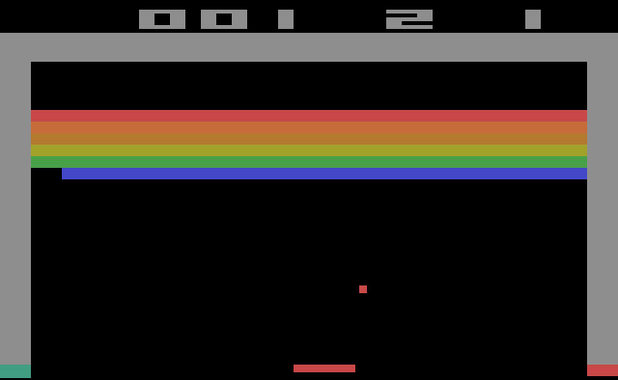
\includegraphics[width=0.99\linewidth]{figs/atari_breakout.jpg}
        \caption{Atari Breakout}
        \label{fig:breakout}
    \end{subfigure}%
    \begin{subfigure}{0.5\textwidth}
        
\includegraphics[width=0.99\linewidth]{figs/atari_breakout_bw.jpg}
        \caption{Black and white Breakout}
        \label{fig:bw_breakout}
    \end{subfigure}
    \caption{Atari Breakout. \ref{fig:breakout} is what Breakout looks like. We have the paddle in the bottom of the screen aiming to hit the ball in order to break the tiles at the top of the screen. \ref{fig:bw_breakout} is our transformation of Atari Breakout into black and white pixels for the purpose of some of the following problems.}
    \label{fig:my_label}
\end{figure}

\begin{parts}
    \part[1] Suppose we are dealing with the black and white version of Breakout\footnote{Play a Google-Doodle version \href{http://goo.gl/hb5xa}{here}} as in Figure~\ref{fig:bw_breakout}. Furthermore, suppose we are representing the state of the game as just a vector of pixel values without considering if a certain pixel is always black or white. Since we are dealing with the black and white version of the game, these pixel values can either be 0 or 1.
    
    What is the size of the state space?\\
    \begin{your_solution}[title = Answer, height=2cm,width=3cm]
        % YOUR ANSWER 
    \end{your_solution}
    
    
    \part[1] In the same setting as the previous part, suppose we wish to apply Q-learning to this problem. What is the size of the Q-value table we will need?\\
    \begin{your_solution}[title =Answer, height=2cm,width=3cm]
        % YOUR ANSWER 
    \end{your_solution}\\
    
    
    
    \part[1] Now assume we are dealing with the colored version of Breakout as in Figure~\ref{fig:breakout}. Now each pixel is a tuple of real valued numbers between $0$ and $1$. For example, black is represented as $(0, 0, 0)$ and white is $(1, 1, 1)$. 
    
    What is the size of the state space and Q-value table we will need?
    \\
    \begin{your_solution}[title=Answer,height=2cm,width=15cm]
        % YOUR ANSWER 
    \end{your_solution}\\
    
    
    % break from here
    By now you should see that we will need a huge table in order to apply Q-learning (and similarly value iteration and policy iteration) to Breakout given this state representation. This table would not even fit in the memory of any reasonable computer! Now this choice of state representation is particularly na\"ive. If we choose a better state representation, we could drastically reduce the table size needed. 
    
    On the other hand, perhaps we don't want to spend our days feature engineering a state representation for Breakout. Instead we can apply function approximation to our reinforcement algorithms! The whole idea of function approximation is that states nearby to the state of interest should have \emph{similar} values. That is, we should be able to generalize the value of a state to nearby and unseen states.
    
    Let us define $q_\pi(s, a)$ as the true action value function of the current policy $\pi$. Assume $q_\pi(s,a)$ is given to us by some oracle. Also define $q(s, a; \wv)$ as the action value predicted by the function approximator parameterized by $\wv$. Here $\wv$ is a matrix of size $\dim(S) \times |\mathcal{A}|$, where $\dim(S)$ denotes the dimension of the state space. Clearly we want to have $q(s, a; \wv)$ be close to $q_\pi(s, a)$ for all $(s, a)$ pairs we see. This is just our standard regression setting. That is, our objective function is just the Mean Squared Error:
    \begin{align}
    J(\wv) = \frac{1}{2} \frac{1}{N} \sum_{s\in\mathcal{S}, a\in\mathcal{A}} \left(q_\pi(s, a) - q(s, a; \wv) \right)^2
    \end{align}
    Because we want to update for each example stochastically\footnote{This isn't really stochastic, you'll be asked in a bit why.}, we get the following update rule:
    \begin{align}
    \wv \leftarrow \wv - \alpha \left(q(s, a; \wv) - q_\pi(s,a) \right) \nabla_\wv q(s, a; \wv)
    \end{align}
    
    However, more often then not\footnote{Always in real life.} we will not have access to the oracle that gives us our target $q_\pi(s, a)$. So how do we get the target to regress $q(s, a; \wv)$ on? One way is to bootstrap\footnote{Metaphorically, the agent is pulling itself up by its own bootstraps.} an estimate of the action value under a greedy policy using the function approximator itself. That is to say
    \begin{align}
    q_\pi (s, a) \approx r + \gamma \max_{a'} q(s', a'; \wv)
    \end{align}
    Where $r$ is the reward observed from taking action $a$ at state $s$, $\gamma$ is the discount factor and $s'$ is the state resulting from taking action $a$ at state $s$. This target is often called the Temporal Difference (TD) target, and gives rise to the following update for the parameters of our function approximator in lieu of a tabular update:
    
    \begin{align}
    \wv \leftarrow \wv - \alpha \bigg( \underbrace{q(s, a; \wv) - \underbrace{\big (r + \gamma \max_{a'}q(s', a'; \wv)\big)}_{\text{TD Target}}}_{\text{TD Error}} \bigg) \nabla_\wv q(s, a; \wv)
    \end{align}
    
    \part[2] Let us consider the setting where we can represent our state by some vector $\sv$, action $a \in \{0, 1, 2\}$ and we choose a linear approximator. That is:
    \begin{align}
    \label{eq:linearEQ}
    q(\sv, a; \wv) = \sv^T\wv_a
    \end{align}
    Again, assume we are in the black and white setting of Breakout as in Figure~\ref{fig:bw_breakout}. Show that tabular Q-learning is just a special case of Q-learning with a linear function approximator by describing a construction of $\sv$. (\textbf{Hint}: Engineer features such that \ref{eq:linearEQ} encodes a table lookup)
    
    \begin{your_solution}[title=Answer,height=6cm,width=15cm]
        % YOUR ANSWER 
    \end{your_solution}
    
    \part[3] Stochastic Gradient Descent works because we can assume that the samples we receive are independent and identically distributed. Is that the case here? If not, why and what are some ways you think you could combat this issue?
    
    \begin{your_solution}[title=Answer,height=4cm,width=15cm]
        % YOUR ANSWER 
    \end{your_solution}
\end{parts}
\end{questions}

\clearpage

\subsection{Empirical Questions}

The following parts should be completed after you work through the programming portion of this assignment (Section \ref{sec:code}). 

\begin{questions}
    \question[4] Run Q-learning on the mountain car environment using both tile and raw features. 
    
    For the raw features: run for 2000 episodes with max iterations of 200, $\epsilon$ set to 0.05, $\gamma$ set to 0.999, and a learning rate of 0.001. 
    
    For the tile features: run for 400 episodes with max iterations of 200, $\epsilon$ set to 0.05, $\gamma$ set to 0.99, and a learning rate of 0.00005.
    
    For each set of features, plot the return (sum of all rewards in an episode) per episode on a line graph. On the same graph, also plot the rolling mean over a 25 episode window. Comment on the difference between the plots.
    
    \begin{your_solution}[title=Plot of Raw, height=10cm,width=15cm]
        % YOUR ANSWER 
        % \begin{center}
        %    \includegraphics[height8.5cm]{allplot.png}
        % \end{center}
    \end{your_solution}
    
    \begin{your_solution}[title=Plot of Tile,height=10cm,width=15cm]
        % YOUR ANSWER 
        % \begin{center}
        %    \includegraphics[height8.5cm]{allplot.png}
        % \end{center}
    \end{your_solution}
    
    \begin{your_solution}[title=Comment,height=5cm,width=15cm]
        % YOUR ANSWER 
    \end{your_solution}
    \clearpage
    \begin{figure}[H]
        \centering
        \begin{subfigure}{0.5\textwidth}
            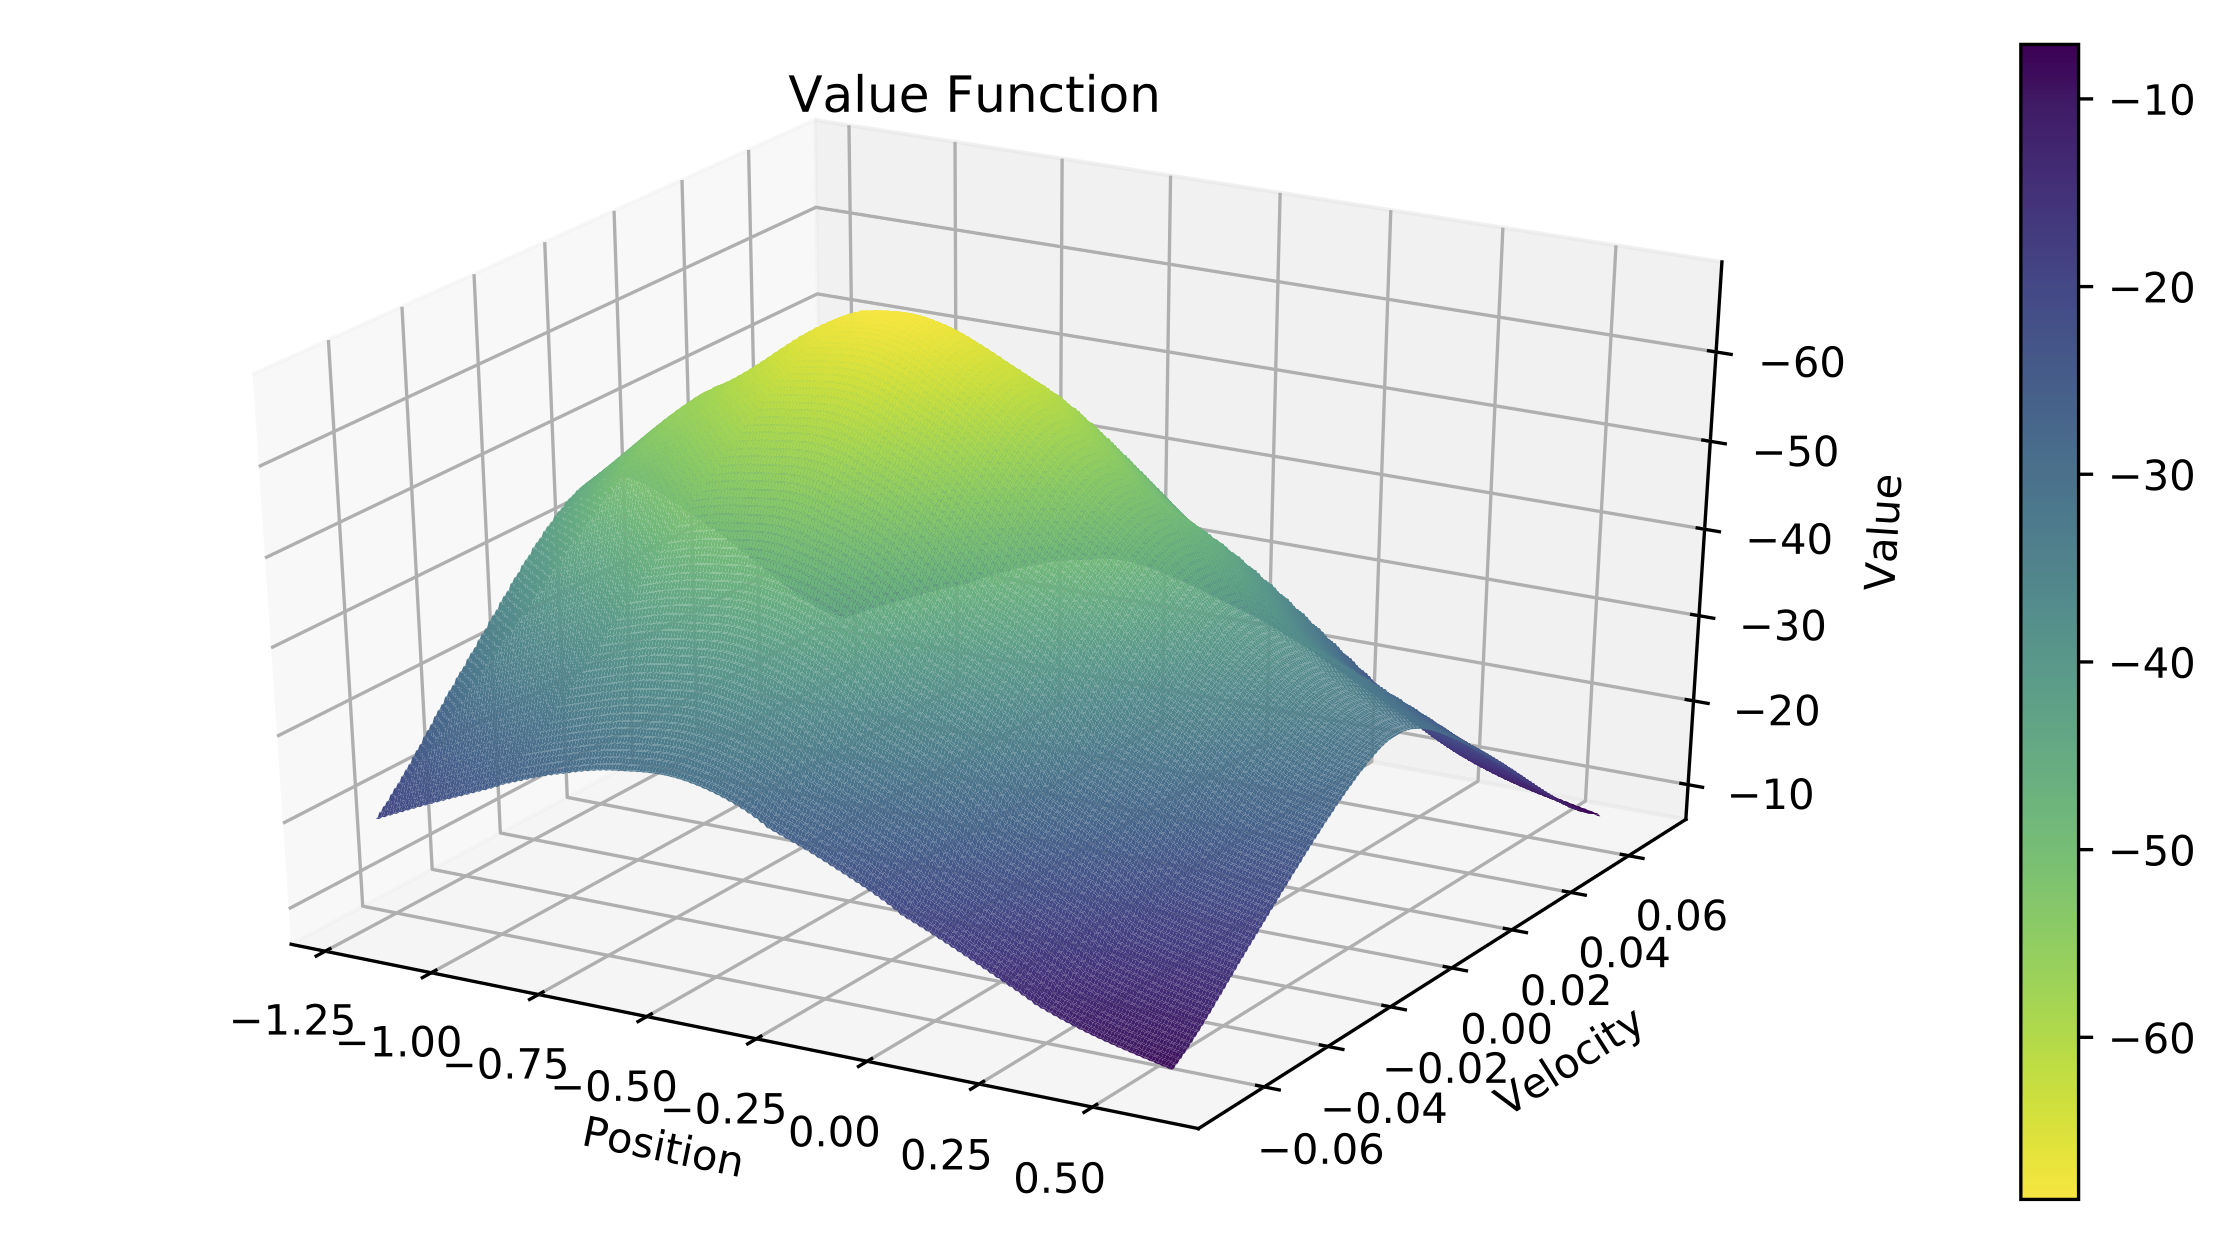
\includegraphics[width=\linewidth]{figs/value_A.png}
            \caption{}
            \label{fig:value_a}
        \end{subfigure}%
        \begin{subfigure}{0.5\textwidth}
            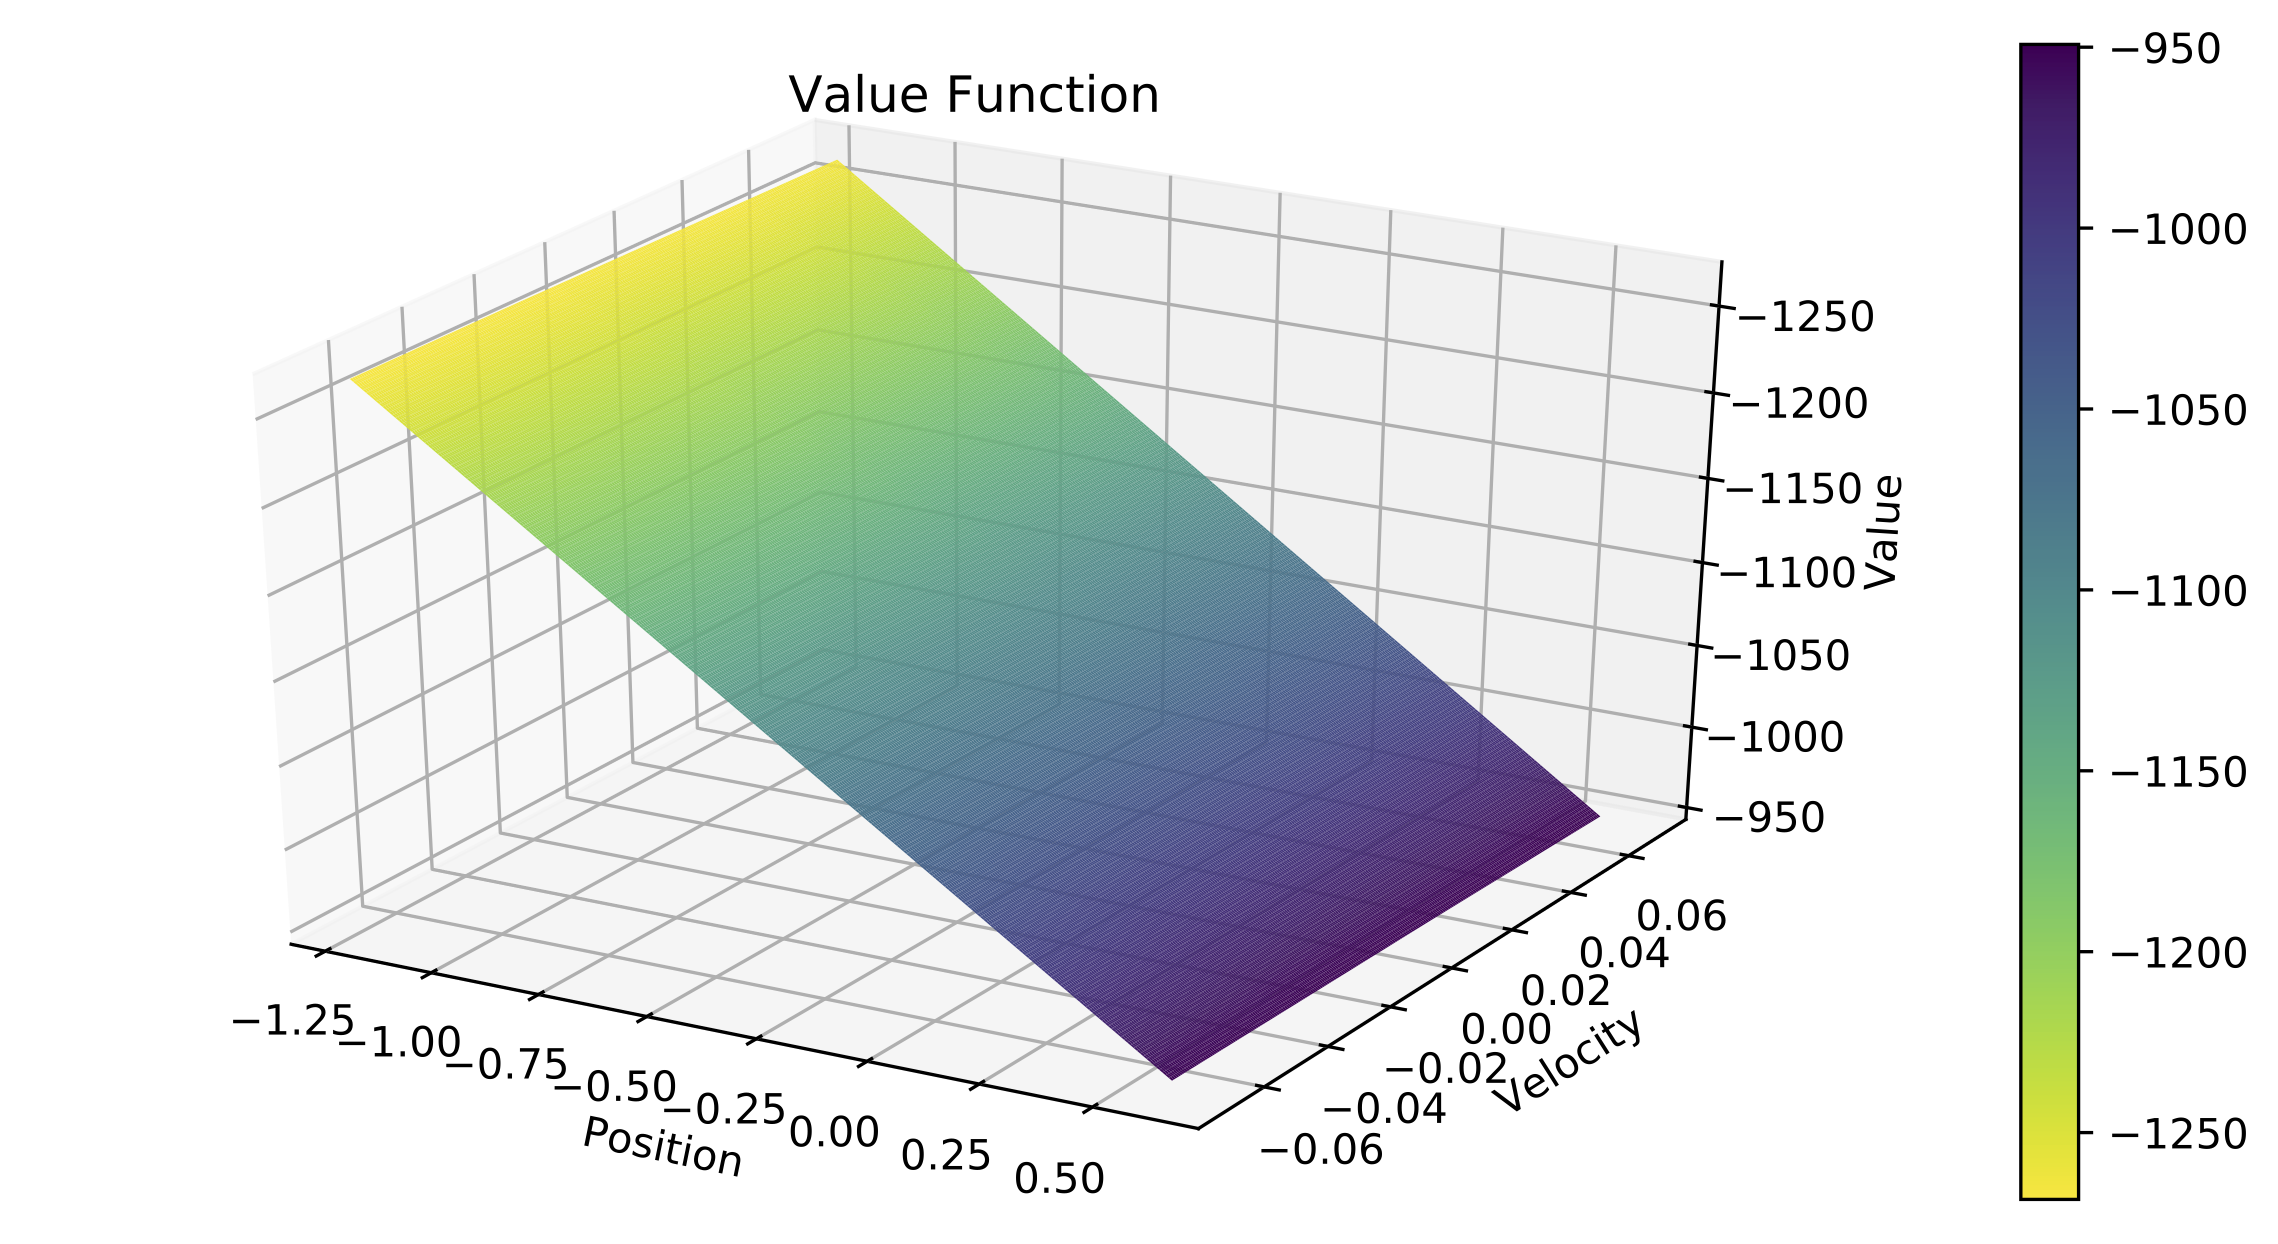
\includegraphics[width=\linewidth]{figs/value_B.png}
            \caption{}
            \label{fig:value_b}
        \end{subfigure}
        \caption{Estimated optimal value function visualizations for both types of features}
        \label{fig:value}
    \end{figure}
    
    \question[2] For both raw and tile features, we have run Q-learning with some good\footnote{For some sense of good.} parameters and created visualizations of the value functions after many episodes. For each plot in Figure~\ref{fig:value}, write down which features (raw or tile) were likely used in Q-learning with function approximation. Explain your reasoning. In addition, interpret each of these plots in the context of the mountain car environment.
    
    \begin{your_solution}[title=Answer,height=5cm,width=15cm]
        % YOUR ANSWER 
    \end{your_solution}

    \question[2] We see that Figure~\ref{fig:value_b} seems to look like a plane. Can the value function depicted in this plot ever be nonlinear? If so, describe a potential shape. If not explain why. (\textbf{Hint:} How do we calculate the value of a state given the Q-values?)

    \begin{your_solution}[title=Answer,height=5cm,width=15cm]
        % YOUR ANSWER 
    \end{your_solution}
    
    
        
    
    \begin{figure}[H]
        \centering
        \begin{subfigure}{0.5\textwidth}
            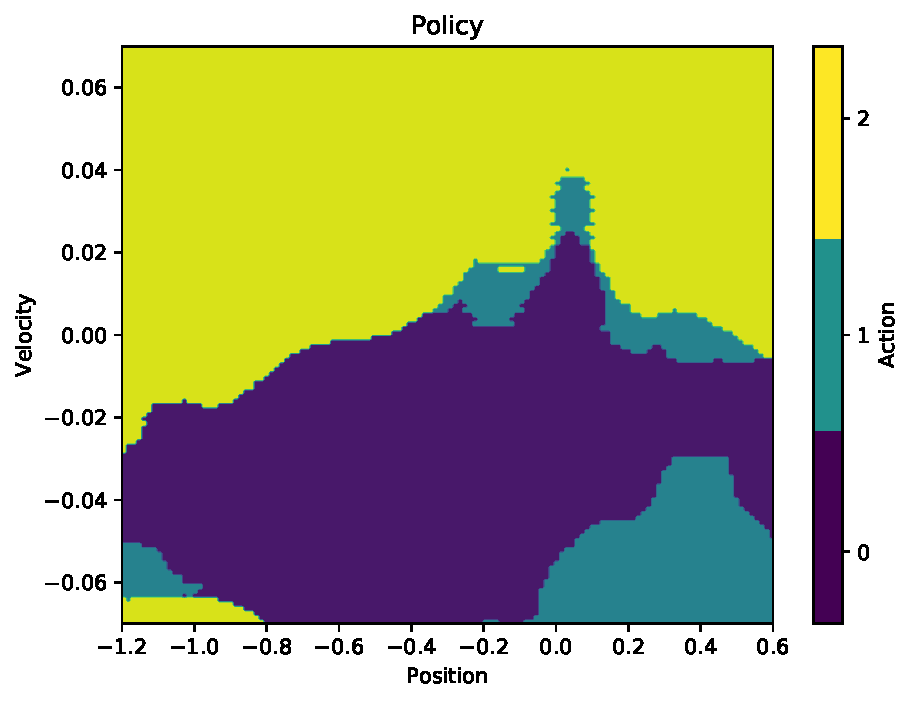
\includegraphics[width=\linewidth]{figs/policy_A.pdf}
            \caption{}
            \label{fig:policy_a}
        \end{subfigure}%
        \begin{subfigure}{0.5\textwidth}
            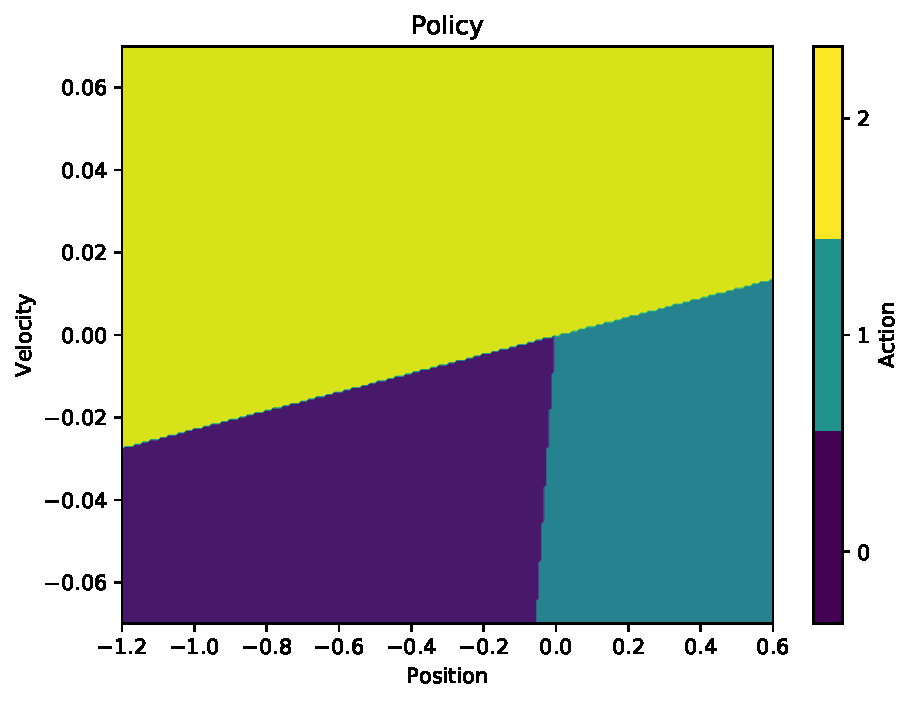
\includegraphics[width=\linewidth]{figs/policy_B.pdf}
            \caption{}
            \label{fig:policy_b}
        \end{subfigure}
        \caption{Estimated optimal policy visualizations for both types of features}
        \label{fig:policy}
    \end{figure}

    \question[2] In a similar fashion to the previous question we have created visualizations of the potential policies learned. For each plot in Figure~\ref{fig:policy} write down which features (raw or tile) were likely used in Q-learning with function approximation. Explain your reasoning. In addition, interpret each of these plots in the context of the mountain car environment. Specifically, why are the edges linear v.s. non-linear? Why do they learn these patches at these specific locations? 
        
    \begin{your_solution}[title=Answer,height=5cm,width=15cm]
        % YOUR ANSWER 
    \end{your_solution}
\end{questions}

    \clearpage
    \clearpage
\section{Programming [68 Points]}
\label{sec:code}

Your goal in this assignment is to implement Q-learning with linear function approximation to solve the mountain car environment. You will implement all of the functions needed to initialize, train, evaluate, and obtain the optimal policies and action values with Q-learning. In this assignment we will provide the environment for you.

The program you write will be automatically graded using the Gradescope system. You may write your program in \textbf{Python, Java, or C++}. However, you should use the same language for all parts below.

\subsection{Specification of Mountain Car}
In this assignment, you will be given code that fully defines the Mountain Car environment. In Mountain Car you control a car that starts at the bottom of a valley. Your goal is to reach the flag at the top right, as seen in Figure~\ref{fig:mountaincar}. However, your car is under-powered and can not climb up the hill by itself. Instead you must learn to leverage gravity and momentum to make your way to the flag. It would also be good to get to this flag as fast as possible.

\begin{figure}[H]
    \centering
    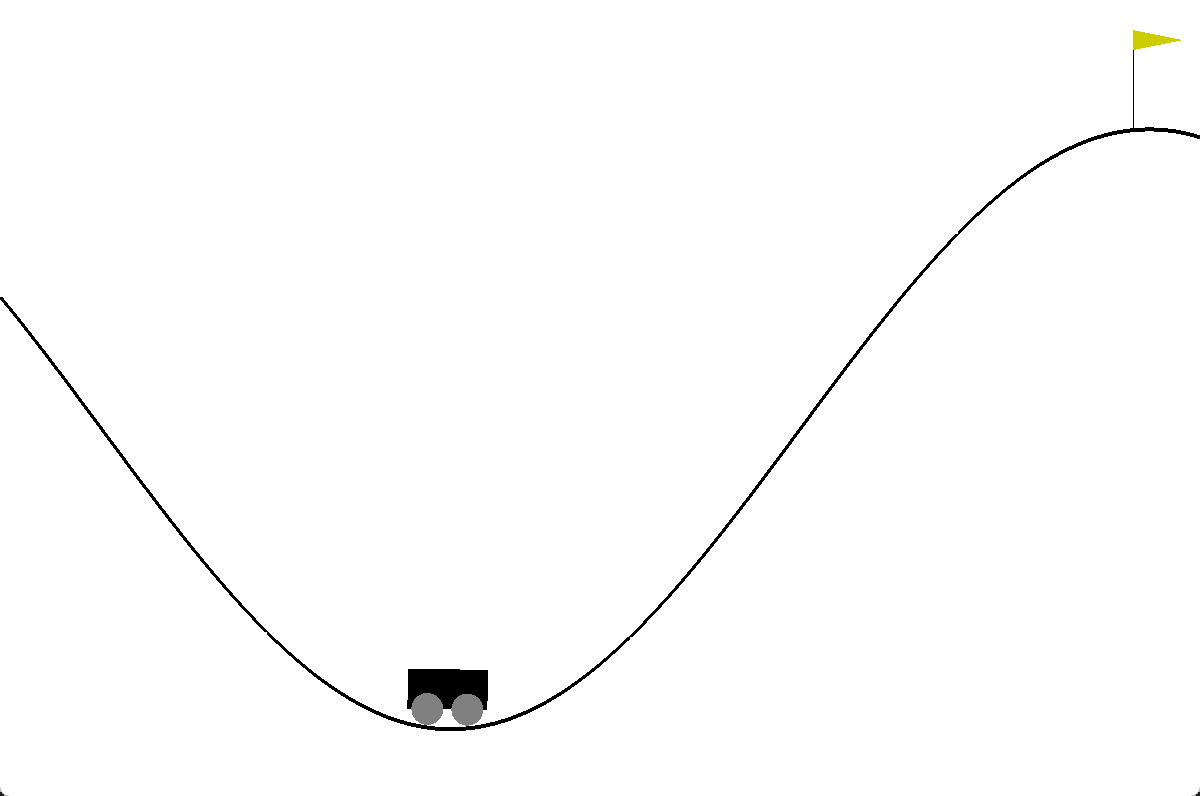
\includegraphics[width=0.5\linewidth]{figs/MountainCar.png}
    \caption{What the Mountain Car environment looks like. The car starts at some point in the valley. The goal is to get to the top right flag.}
    \label{fig:mountaincar}
\end{figure}

The state of the environment is represented by two variables, \texttt{position} and \texttt{velocity}.\\\texttt{position} can be between $[-1.2, 0.6]$ (inclusive) and \texttt{velocity} can be between $[-0.07, 0.07]$ (inclusive). These are just measurements along the $x$-axis.

The actions that you may take at any state are $\{0, 1, 2\}$, where each number corresponds to an action: (0) pushing the car left, (1) doing nothing, and (2) pushing the car right.

\subsection{Q-learning With Linear Approximations}
The Q-learning algorithm is a model-free reinforcement learning algorithm, where we assume we don't have access to the model of the environment the agent is interacting with. We also don't build a complete model of the environment during the learning process. A learning agent interacts with the environment solely based on calls to \textbf{step} and \textbf{reset} methods of the environment. Then the Q-learning algorithm updates the q-values based on the values returned by these methods. Analogously, in the approximation setting the algorithm will instead update the parameters of q-value approximator.


Let the learning rate be $\alpha$ and discount factor be $\gamma$. Recall that we have the information after one interaction with the environment, $(s, a, r, s')$. The tabular update rule based on this information is: 
\[
    Q(s,a) = (1 - \alpha) Q(s, a) + \alpha \left(r + \gamma \max_{a'} Q(s', a')\right)
\]

Instead, for the function approximation setting we use the following update rule derived from the Function Approximation Section\footnote{Note that we have made the bias term explicit here, where before it was implicitly folded into $\wv$ }:

\[
\wv \leftarrow \wv - \alpha \left(q(\sv, a; \wv) - (r + \gamma \max_{a'} q(\sv', a'; \wv)\right) \nabla_\wv q(\sv, a; \wv)
\]
Where:
\[
q(\sv,a;\wv) = \sv^T \wv_a + b
\]
The epsilon-greedy action selection method selects the optimal action with probability $1 - \epsilon$ and selects uniformly at random from one of the 3 actions (0, 1, 2) with probability $\epsilon$. The reason that we use an epsilon-greedy action selection is we would like the agent to do explorations by stochastically selecting random actions with small probability. For the purpose of testing, we will test two cases: $\epsilon = 0$ and $0 < \epsilon < 1$. When $\epsilon = 0$ (no exploration), the program becomes deterministic and your output have to match our reference output accurately. In this case, \textbf{pick the action represented by the smallest number if there is a draw in the greedy action selection process}. For example, if we're at state $s$ and $Q(s, 0) = Q(s, 2)$, then take action $0$. When $0 < \epsilon < 1$, your output will need to fall in a certain range within the reference determined by running exhaustive experiments on the input parameters.


\subsection{Feature Engineering}
Linear approximations are great in their ease of use and implementations. However, there sometimes is a downside; they're \emph{linear}. This can pose a problem when we think the value function itself is nonlinear with respect to the state. For example, we may want the value function to be symmetric about 0 velocity. To combat this issue we could throw a more complex approximator at this problem, like a neural network. But we want to maintain simplicity in this assignment, so instead we will look at a nonlinear transformation of the ``raw'' state.

\begin{figure}[H]
\centering
\begin{subfigure}{0.5\textwidth}

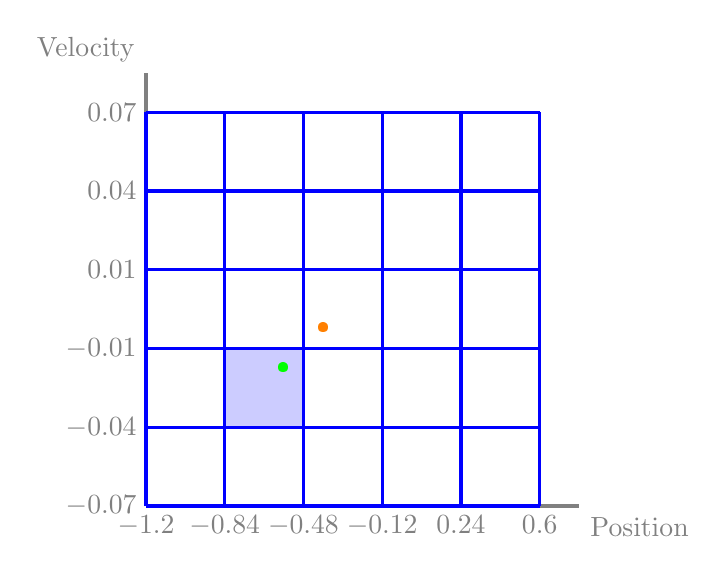
\begin{tikzpicture}[scale=1.0]
% https://tex.stackexchange.com/questions/45808/tikz-grid-lines
% https://tex.stackexchange.com/questions/305138/modify-the-scale-of-x-axis-and-y-axis
\pgfkeys{/pgf/number format/.cd,fixed,precision=2}
% Draw labels
\draw [ultra thick,gray,] (0,0)--(5.5,0) node[below right] {\text{Position}};
\draw [ultra thick,gray,] (0,0)--(0,5.5) node[above left] {\text{Velocity}};
% Draw axis
\newcommand*{\xMin}{0}%
\newcommand*{\xMax}{5}%
\newcommand*{\yMin}{0}%
\newcommand*{\yMax}{5}%
    \foreach \i in {\xMin,...,\xMax} {
        \draw [very thin,gray] (\i,\yMin) -- (\i,\yMax)  node [below] at (\i,\yMin) {\pgfmathparse{(\i/50)*18-1.2}$\pgfmathprintnumber{\pgfmathresult}$};
    }
    \foreach \i in {\yMin,...,\yMax} {
        \draw [very thin,gray] (\xMin,\i) -- (\xMax,\i) node [left] at (\xMin,\i) {\pgfmathparse{(\i/500)*14-0.07}$\pgfmathprintnumber{\pgfmathresult}$};
    }
% Draw grids
\draw [step=1.0,blue, very thick] (0.0,0.0) grid (5.0,5.0);
% \draw [very thick, red, step=1.0cm,xshift=-0.5cm, yshift=-0.5cm] (0.5,0.5) grid +(5.0,5.0);

% Draw shaded regions
\fill [blue, opacity=0.2] (1,1) rectangle (2,2);
% \fill [red, opacity=0.2] (1.5,1.5) rectangle (2.5,2.5);

% Draw point
\node [green] at (1.75,1.75) {\textbullet};
\node [orange] at (2.25, 2.25) {\textbullet};

\end{tikzpicture}
\caption{A discretization of the state space of Mountain Car}
\label{fig:discrete}
\end{subfigure}%
\begin{subfigure}{0.5\textwidth}

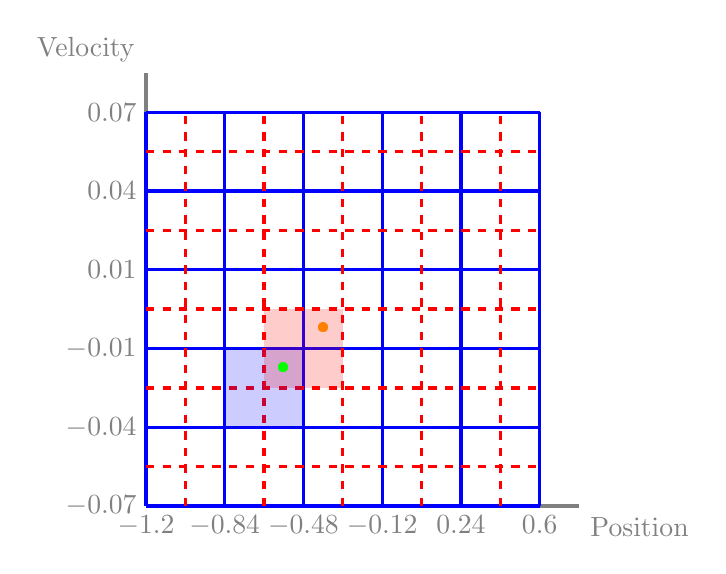
\begin{tikzpicture}[scale=1.0]
% https://tex.stackexchange.com/questions/45808/tikz-grid-lines
% https://tex.stackexchange.com/questions/305138/modify-the-scale-of-x-axis-and-y-axis
\pgfkeys{/pgf/number format/.cd,fixed,precision=2}
% Draw labels
\draw [ultra thick,gray,] (0,0)--(5.5,0) node[below right] {\text{Position}};
\draw [ultra thick,gray,] (0,0)--(0,5.5) node[above left] {\text{Velocity}};
% Draw axis
\newcommand*{\xMin}{0}%
\newcommand*{\xMax}{5}%
\newcommand*{\yMin}{0}%
\newcommand*{\yMax}{5}%
    \foreach \i in {\xMin,...,\xMax} {
        \draw [very thin,gray] (\i,\yMin) -- (\i,\yMax)  node [below] at (\i,\yMin) {\pgfmathparse{(\i/50)*18-1.2}$\pgfmathprintnumber{\pgfmathresult}$};
    }
    \foreach \i in {\yMin,...,\yMax} {
        \draw [very thin,gray] (\xMin,\i) -- (\xMax,\i) node [left] at (\xMin,\i) {\pgfmathparse{(\i/500)*14-0.07}$\pgfmathprintnumber{\pgfmathresult}$};
    }
% Draw grids
\draw [step=1.0,blue, very thick] (0.0,0.0) grid (5.0,5.0);
\draw [very thick, dashed, red, step=1.0cm,xshift=-0.5cm, yshift=-0.5cm] (0.5,0.5) grid +(5.0,5.0);

% Draw shaded regions
\fill [blue, opacity=0.2] (1,1) rectangle (2,2);
\fill [red, opacity=0.2] (1.5,1.5) rectangle (2.5,2.5);

% Draw point
\node [green] at (1.75,1.75) {\textbullet};
\node [orange] at (2.25, 2.25) {\textbullet};

\end{tikzpicture}
\caption{A tiling of the state space of Mountain Car}
\label{fig:tiling}
\end{subfigure}

\caption{State representations for the states of Mountain Car}
\label{fig:states}
\end{figure}

For the Mountain Car environment, we know that \texttt{position} and \texttt{velocity} are both bounded. What we can do is draw a grid over the possible \texttt{position}-\texttt{velocity} combinations as seen in Figure~\ref{fig:discrete}. We then enumerate the grid from bottom left to top right, row by row. Then we map all states that fall into a grid square with the corresponding one-hot encoding of the grid number. For efficiency reasons we will just use the index that is non-zero. For example the green point would be mapped to $\{6\}$ and the orange point to $\{12\}$. This is called a \emph{discretization} of the state space.

The downside to the above approach is that although observing the green point will let us learn parameters that generalize to other points in the shaded blue region, we will not be able to generalize to the orange point even though it is nearby. We can instead draw two grids over the state space, each offset slightly from each other as in Figure~\ref{fig:tiling}. Now we can map the green point to two indices, one for each grid, and get $\{6, 39\}$ (note the index for orange grid starts from the end of blue index, i.e. 25). Now the green point has parameters that generalize to points that map to $\{6\}$ (the blue shaded region) in the first discretization and parameters that generalize to points that map to $\{39\}$ (the red shaded region) in the second. We can generalize this to multiple grids, which is what we do in practice. This is called a \emph{tiling} or a \emph{coarse-coding} of the state space. 


\subsection{Implementation Details}
Here we describe the API to interact with the Mountain Car environment available to you in Python. The other languages will have an analagous API. 

\begin{itemize}
    \item \texttt{\_\_init\_\_(mode, fixed)}: Initializes the environment to the a mode specified by the value of \texttt{mode}. This can be a str ing of either ``raw'' or ``tile''. 
    
    ``raw'' mode tells the environment to give you the state representation of raw features encoded in a sparse format: $\{0 \rightarrow \texttt{position}, 1 \rightarrow \texttt{velocity}\}$.
    
    In ``tile'' mode you are given indices of the tiles which are active in a sparse format: $\{T_1 \rightarrow 1, T_2 \rightarrow 1, \ldots T_n \rightarrow 1\}$ where $T_i$ is the tile index for the $i$th tiling. All other tile indices are assumed to map to 0. For example the state representation of the example in Figure~\ref{fig:tiling} would become $\{6 \rightarrow 1, 39 \rightarrow 1\}$.
    
    The dimension of the state space of the ``raw'' mode is 2. The dimension of the state space of the ``tile'' mode is 2048. These values can be accessed from the environment through the \texttt{state\_space} property, and similarly for other languages.
    
    \texttt{fixed} is an optional argument for debugging. See Section 1.5 for more details.
    
    \item \texttt{reset()}: Reset the environment to starting conditions.
    \item \texttt{step(action)}: Take a step in the environment with the given action. \texttt{action} must be either $0$, $1$ or $2$. This will return a tuple of $(\texttt{state}, \texttt{reward}, \texttt{done})$ which is the next state, the reward observed, and a boolean indicating if you reached the goal or not, ending the episode. The \texttt{state} will be either a raw' or tile representation, as defined above, depending on how you initialized Mountain Car.  If you observe \texttt{done = True} then you should \texttt{reset} the environment and end the episode. Failure to do so will result in undefined behavior.
    \item \textbf{[Python Only]} \texttt{render(self)}: Optionally render the environment. It is computationally intensive to render graphics, so only render a full episode once every 100 or 1000 episodes. Requires the installation of \texttt{pyglet}. This will be a no-op in Gradescope.
\end{itemize}

You should now implement your Q-learning algorithm with linear approximations as \newline\texttt{q\_learning.\{py|java|cpp\}}. The program will assume access to a given environment file(s) which contains the Mountain Car environment which we have given you.  \textbf{Initialize the parameters of the linear model with all 0 (and don't forget to include a bias!) and use the epsilon-greedy strategy for action selection.}

Your program should write a output file containing the total rewards (the returns) for every episode after running Q-learning algorithm. There should be one return per line.

Your program should also write an output file containing the weights of the linear model. The first line should be the value of the bias. Then the following $|\mathcal{S}| \times |\mathcal{A}|$ lines should be the values of weights, outputted in row major order\footnote{\url{https://en.wikipedia.org/wiki/Row-_and_column-major_order}}, assuming your weights are stored in a $|\mathcal{S}| \times |\mathcal{A}|$ matrix.

The autograder will use the following commands to call your function:

\begin{tabbing}
For Python: \=\texttt{\$ \textbf{python} q\_learning.\textbf{py} [args\dots]}\\
For Java: \>\texttt{\$ \textbf{javac} -cp "./lib/ejml-v0.33-libs/*:./" q\_learning.\textbf{java}};\\ \>  \texttt{\textbf{java} -cp "./lib/ejml-v0.33-libs/*:./" q\_learning [args\dots]}\\
For C++: \>\texttt{\$ \textbf{g++} -g -std=c++11 -I./lib q\_learning.\textbf{cpp}; ./a.out [args\dots]}\\
% For Octave: \>\texttt{\$ \textbf{octave} -qH q\_learning.\textbf{m} [args\dots]}
\end{tabbing}

Where above \texttt{[args\dots]} is a placeholder for command-line arguments: \texttt{<mode>} \texttt{<weight\_out>} \texttt{<returns\_out>} \texttt{<episodes>} \texttt{<max\_iterations>} \texttt{<epsilon>} \texttt{<gamma>} \texttt{<learning\_rate>}. These arguments are described in detail below:
\begin{enumerate}
    \item \texttt{<mode>}: mode to run the environment in. Should be either \texttt{``raw''} or \texttt{``tile''}.
    \item \texttt{<weight\_out>}: path to output the weights of the linear model.
    \item \texttt{<returns\_out>}: path to output the returns of the agent
    \item \texttt{<episodes>}: the number of episodes your program should train the agent for. One episode is a sequence of states, actions and rewards, which ends with terminal state or ends when the maximum episode length has been reached.
    \item \texttt{<max\_iterations>}: the maximum of the length of an episode. When this is reached, we terminate the current episode.
    \item \texttt{<epsilon>}: the value $\epsilon$ for the epsilon-greedy strategy
    \item \texttt{<gamma>}: the discount factor $\gamma$.
    \item \texttt{<learning\_rate>}: the learning rate $\alpha$ of the Q-learning algorithm
\end{enumerate}


Example command for python users:
\begin{lstlisting}[language=Shell]
$ python q_learning.py raw weight.out returns.out \ 
 4 200 0.05 0.99 0.01
\end{lstlisting}

Example output from running the above command (your code won't match exactly, but should be close).

\texttt{<weight\_out>}
\begin{lstlisting}
-7.6610506220312296
1.3440159024460183
1.344872959883069
1.340055578403996
-0.0007770480987990149
0.0011306483117300896
0.0017559989206646666
\end{lstlisting}

\texttt{<returns\_out>}
\begin{lstlisting}
-200.0
-200.0
-200.0
-200.0
\end{lstlisting}


\subsection{Debugging Tips}

To help with debugging, we have provided the option for fixing the initialization of Mountain Car. To utilize this option, provide the additional argument \texttt{fixed = 1} when initializing Mountain Car. In this setup, the Mountain Car is initialized with \texttt{position = 0.8} and \texttt{velocity = 0}. 

We recommend to first run your program with the most simple parameters and check the outputs against manually calculated values. Remember to set \texttt{<epsilon>=0} so the program is run without epsilon-greedy strategy.

Example command for python users: 
\begin{lstlisting}[language=Shell]
$ python q_learning.py raw simple_weight.out simple_returns.out \
1 1 0.0 1 1
\end{lstlisting}
Once your program works, you can change one of the parameters to be slightly more complex, e.g. set \texttt{<max\_iterations>=2} or \texttt{<gamma>=0.9}, and check with your manual calculations again.

In addition, we have provided \texttt{fixed\_weight.out} and \texttt{fixed\_returns.out} in the handout, which are generated using the following parameters:
\begin{itemize}
    \item \texttt{<mode>}: \texttt{``tile''}
    \item \texttt{<episodes>}: \texttt{25}
    \item \texttt{<max\_iterations>}: \texttt{200}
    \item \texttt{<epsilon>}: \texttt{0.0}
    \item \texttt{<gamma>}: \texttt{0.99}
    \item \texttt{<learning\_rate>}: \texttt{0.005}
\end{itemize}

Example command for python users:
\begin{lstlisting}[language=Shell]
$ python q_learning.py tile fixed_weight.out fixed_returns.out \ 
 25 200 0.0 0.99 0.005
\end{lstlisting}

Your output should match with the reference up till the last 4 digits.

\textbf{Before submitting to Gradescope, do not forget to remove the \texttt{fixed} argument when initializing Mountain Car. }

Some additional tips: If you get a \texttt{"ValueError: high is out of bounds for int32"} this is due to python version differences. You can either update your python or change the dtype of the randint function to int64. This can be done by changing line 18 to
\begin{verbatim}
    seed = rng.randint(2**32 - 1, dtype=np.int64)
\end{verbatim}


\subsection{Gradescope Submission}

You should submit your \texttt{q\_learning.\{py|java|cpp\}} to Gradescope.
Note: please do not use other file names. This will cause problems for the autograder to correctly detect and run your code.

Note: For this assignment, you may make upto 30 submissions to Gradescope before the deadline, but only your last submission will be graded.

\newpage
\section{Collaboration Questions}
After you have completed all other components of this assignment, report your answers to these questions regarding the collaboration policy. Details of the policy can be found \href{http://www.cs.cmu.edu/~mgormley/courses/10601/syllabus.html}{here}.
\begin{enumerate}
    \item Did you receive any help whatsoever from anyone in solving this assignment? If so, include full details.
    \item Did you give any help whatsoever to anyone in solving this assignment? If so, include full details.
    \item Did you find or come across code that implements any part of this assignment ? If so, include full details.
\end{enumerate}

\begin{your_solution}[height=6cm]
% YOUR ANSWER 

\end{your_solution}
\end{document}
